\documentclass[a4paper]{article}
 
\usepackage[margin=1in]{geometry}
\usepackage{amsmath,amsthm,amssymb,bbm,wasysym}
\usepackage[czech]{babel}
\usepackage[utf8]{inputenc}
\usepackage[T1]{fontenc}
\usepackage{tikz}
\usepackage{graphicx}
\usepackage{enumitem}
\usepackage{tabto}
\usepackage{amsmath}

\graphicspath{ {./} }

\DeclareMathOperator{\Ex}{\mathbb{E}} % střední hodnota X pomocí $\Ex X$

\newcommand{\N}{\mathbb{N}} % přirozená čísla
\newcommand{\Z}{\mathbb{Z}} % celá čísla
\newcommand{\R}{\mathbb{R}} % reálná čísla

\renewcommand{\qed}{\hfill\blacksquare} % Quod Est Demonstratum (QED) 

% tohle je pro prostředí úkolů
\newenvironment{ukol}[2][]{\begin{trivlist} 
\item[\hskip \labelsep {\bfseries #1}\hskip \labelsep {\bfseries #2}]}{\end{trivlist}}

\linespread{1.15}
 
\begin{document}
 
% --------------------------------------------------------------
%                         Začni ZDE
% --------------------------------------------------------------
 
\title{ Evoluční algoritmy \\ 2. domácí úkol
        } 
\author{Martin Gráf}
\date{19.4.2023}

\maketitle

Úkolem bylo sestavit malý dataset tvořený z desítek obrázků od alespoň (a v našem případě právě) 5 kategorií. Výsledný dataset je použit k trénování zvoleného modelu konvoluční sítě - Konkrétně ResNet50 v našem případě - a jeho validaci.

\begin{ukol}{Dataset}
\begin{itemize}
	\item Dataset byl shromážděn pomocí automatického Web Crawlera, který stáhnul právě 70 výsledků obrázkového vyhledávání prohlížeče Bing - Důvod použití Bing je prostý. Google API pro podobnou akci je buď deprecated, nebo rozbité. K tomuto účelu jsme použili Python package \textbf{bing\_image\_downloader}. Takto získané obrázky jsme následně byli nuceni manuálně projít a odstranit duplicitní či nerelevantní obrázky. Vyhledávač přeci jen negarantuje pouze relevantní výsledky. Tímto způsobem jsme získali celkem 42 různých fotek všech 5 kategorií - Kokain, extáze, crack, methamphetamine, a marihuana.
	\item \begin{center}
		\begin{tabular}{ c c c c c }
		 \includegraphics[width=.18\linewidth]{./dataset/cocaine/Image_1} & \includegraphics[width=.18\linewidth]{./dataset/cocaine/Image_2} & \includegraphics[width=.18\linewidth]{./dataset/cocaine/Image_3} & \includegraphics[width=.18\linewidth]{./dataset/cocaine/Image_4} & \includegraphics[width=.18\linewidth]{./dataset/cocaine/Image_5} \\ 
		 \includegraphics[width=.18\linewidth]{./dataset/crack drug/Image_1} & \includegraphics[width=.18\linewidth]{./dataset/crack drug/Image_2} & \includegraphics[width=.18\linewidth]{./dataset/crack drug/Image_3} & \includegraphics[width=.2\linewidth]{./dataset/crack drug/Image_7} & \includegraphics[width=.2\linewidth]{./dataset/crack drug/Image_8} \\  
		\includegraphics[width=.18\linewidth]{./dataset/ecstasy drug/Image_1} & \includegraphics[width=.18\linewidth]{./dataset/ecstasy drug/Image_4} & \includegraphics[width=.18\linewidth]{./dataset/ecstasy drug/Image_3} & \includegraphics[width=.18\linewidth]{./dataset/ecstasy drug/Image_7} & \includegraphics[width=.18\linewidth]{./dataset/ecstasy drug/Image_6} \\  
		\includegraphics[width=.18\linewidth]{./dataset/methamphetamine/Image_1} & \includegraphics[width=.18\linewidth]{./dataset/methamphetamine/Image_4} & \includegraphics[width=.18\linewidth]{./dataset/methamphetamine/Image_3} & \includegraphics[width=.18\linewidth]{./dataset/methamphetamine/Image_7} & \includegraphics[width=.18\linewidth]{./dataset/methamphetamine/Image_6} \\  
		\includegraphics[width=.18\linewidth]{./dataset/weed/Image_1} & \includegraphics[width=.18\linewidth]{./dataset/weed/Image_4} & \includegraphics[width=.18\linewidth]{./dataset/weed/Image_5} & \includegraphics[width=.18\linewidth]{./dataset/weed/Image_7} & \includegraphics[width=.18\linewidth]{./dataset/weed/Image_6} \\  
		\end{tabular}
		\end{center}
	\item Typické aplikace počítačového vidění a klasifikace obrázků vidíme hlavně v dopravě a logistice, častěji a častěji se ale používá i v oblasti bezpečnosti. Klasifikátor schopný rozeznat různé typy drog na základě tvarů, barev, nebo i kontextu v jakém jsou často viděny by tak mohl mít aplikace při detekci substancí buďto u kamer na veřejných místech, nebo u bezpečnostních checkpointů jako třeba na letištích. Existuje ale jedna snad nedostatečně využitá aplikace takového klasifikátoru: Harm reduction. Vznikl-li by veřejně dostupný nástroj - například formou mobilní aplikace - schopný rychlého rozeznání různých typů drog, poskytnutí rad k bezpečnému užití a varování před možnými nežádoucími účinky a nebezpečnými dávkami či kombinacemi, nebo dokonce schopný identifikace možných nečistot, uživatelé nelegálních substancí by získali extra vrstvu ochrany před potenciálním nebezpečím.
	\item Dataset obsahuje právě 5 populárních drog. Tyto drogy jsou od sebe s vyjímkou cracku a kokainu poměrně snadno rozlišitelné (Crack a kokain jsou vlastně stejnou drogou v různých formách - Crack je zpracovaný do formy míněné ke kouření, kdežto kokain je míněný k rozpuštění či přímé inhalaci). Pracujeme tedy s obrázky Kokainu, Cracku, Extáze, Marihuany, a Methamphetaminu, neboli populárního českého "perníku".
	\item Ke každé třídě máme 42 obrázků, 35 z těchto obrázků bude použito ke trénování, 7 k validaci.
	\item Zvolená konvoluční síť - ResNet50 - pracuje s velikostmi obrázků 224.
	\item S obrázky nebylo třeba provádět žádné další akce. Museli jsme je pouze manuálně očistit od nerelevantních dat.
\end{itemize}

\end{ukol}

\begin{ukol}{Modely}
\begin{itemize}
	\item Zvolili jsme model ResNet50, zejména díky jeho snadné rozšířitelnosti a malé velikosti. Model se dělí do stejných segmentů, z nichž žádný není nutně závislý na předešlém. Model je tak připravený na snadné rozšíření.
	\item Z ResNet50 tak stačilo odstranit output vrstvu pomocí \textit{include\_top=False}. To nám dovolilo připojit naše modifikace namísto outputu bez dalších komplikací.
	\item Konečný model je sekvenční, kde první vrstvou je celý ResNet50 model s uříznutou hlavičkou. Tento model je sám o sobě poměrně spolehlivý a data je schopný zpracovat bez větší intervence, naše úpravy tak stačí směřovat na zpracování výstupu.
	\item Připojené vrstvy jsou \textbf{MaxPooling2D} k redukci velikosti výstupu, vrstvou \textbf{Flatten} zredukujeme jeho dimenzi, a následně použijeme 2* vrstvu \textbf{Dense} abychom získali požadovaný počet outputů.
	\item Model konečně využívá ztrátovou funkci \textbf{SparseCategoricalCrossentropy} neboť chceme výstup jako vektor pravděpodobností každé kategorie, a optimizer \textbf{RMSprop}.
	\item Je nutno podotknout, že jsme zamkli trénování modelu ResNet50, ale dovolili trénování námi přidaných vrstev. Také podotkneme, že zmíněné vrstvy jsou spojeny v rámci Sekvenčního modelu.
	\item \textbf{Pro porovnání} jsme také vyzkoušeli a změřili \textbf{Neupravený ResNet50} a \textbf{jednoduchý model ze cvičení}. ResNet50 jsme tentokrát použili i s output layerem a povolili trénování celé sítě, a zkompilovali za použití stejných metrik a optimalizací jako předchozí upravený model. Ze cvičení jsme převzali jednoduchou konvoluční síť pro porovnání, opět za použití stejných metrik.
\end{itemize}

\end{ukol}

\begin{ukol}{Výsledky}
\begin{itemize}
	\item ResNet50 samotný byl sice ozkoušen, nevedl ovšem k dobrým výsledkům neboť drogy klasifikovat neumí, proto prezentujeme výsledky jenom pro naši upravenou verzi.
	\item \begin{center}
		\begin{tabular}{ c c c }
		Model & Trénovací accuracy & Testovací accuracy \\ 
		Upravený ResNet50 & 0.9762 & 0.8095  \\
		Neupravený ResNet50 & 0.9464 & 0.6429 \\
		Jednoduchý model & 0.6071 & 0.2143
		\end{tabular}
		\end{center}
	\item 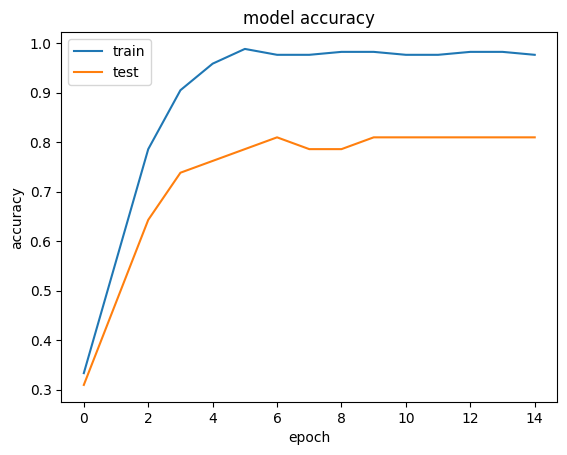
\includegraphics{accuracy}
	\item 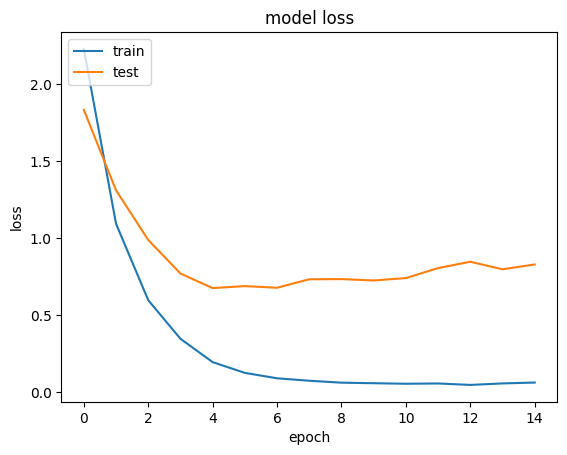
\includegraphics{loss}
\end{itemize}

\end{ukol}

\end{document}
